% \documentclass[12pt]{scrreprt}
\documentclass[12pt]{report} 

% language may be romanian or english (default is english)
% type may be bachelor or master (default is bachelor)
\usepackage[language=english, type=bachelor]{style}

%\geometry{a4paper,top=2.5cm,left=3cm,right=2.5cm,bottom=2.5cm}
%in style
%controlling the appearance of your headers and footers
\usepackage{fancyhdr}
\captionsetup[figure]{font=footnotesize}
\pagestyle{fancy}
\lhead{}
\chead{}
\renewcommand{\headrulewidth}{0.2pt}
\renewcommand{\footrulewidth}{0.2pt}
\setlength{\headheight}{14.5pt}

\begin{document}

\specialization{INFORMATICĂ ENGLEZĂ}
\title{From Sound to Light: A Real-Time System for Generative Stage Lighting via Music Information Retrieval}			   
\author{Apăvăloaiei Alexandru}								
\supervisor{Lect. Nechita Mihai}			
				
\maketitle


\newpage
\thispagestyle{empty}
\mbox{}
\newpage
\pagenumbering{roman} 

\cleardoublepage
ABSTRACT (EN)
\vspace{0.5cm}	
\hrule
\vspace{0.5cm}	
%\cleardoublepage

This thesis presents the design and development of a real-time generative stage-lighting system that transforms musical input into synchronized visual output. The work is situated at the intersection of Music Information Retrieval, automatic stage lighting control, real-time audio processing, and interactive web-based 3D rendering. It builds on MIR techniques for extracting meaningful information from music, including rhythm and audio features, and applies them to a sound-to-light pipeline in which musical analysis directly drives lighting behavior.

Chapter~\ref{chap:theoretical-background} introduces the audio, musical, perceptual, and machine-learning foundations required by the system, from digital audio representation and beat tracking to music-colour associations, automated stage lighting control, real-time processing, and sequence-to-sequence architectures. Chapter~\ref{chap:technologies-and-platform-constraints} evaluates the web as a platform for real-time audio-visual applications, including WebGL, Three.js, the Web Audio API, machine-learning deployment, React, React Three Fiber, and the platform constraints that shape the prototype. Chapter~\ref{chap:methodology-requirements-system-design} defines the methodological approach, requirements, hybrid architecture, runtime data flow, and latency-aware pipeline of the system.

The main personal contribution is the integration of research-oriented MIR and generative lighting models into an interactive application that can operate as a practical real-time prototype. The system combines browser-based audio capture and 3D rendering with a Python inference server running beat tracking and Skip-BART, connected through WebSocket communication and shared frontend state. Its originality lies not in proposing a new MIR model, but in designing and implementing a coherent sound-to-light application that turns existing models into a responsive creative tool, with explicit attention to usability, latency, architecture, and expressive music-visual mapping.

\cleardoublepage
ABSTRACT (RO)
\vspace{0.5cm}
\hrule
\vspace{0.5cm}

Această lucrare prezintă proiectarea și dezvoltarea unui sistem generativ de iluminat scenic în timp real, care transformă intrarea muzicală în ieșire vizuală sincronizată. Lucrarea este situată la intersecția dintre Music Information Retrieval, controlul automat al iluminatului scenic, procesarea audio în timp real și randarea 3D interactivă bazată pe web. Ea se bazează pe tehnici MIR pentru extragerea informațiilor relevante din muzică, inclusiv ritm și trăsături audio, și le aplică într-un flux sunet-lumină în care analiza muzicală conduce direct comportamentul luminilor.

Capitolul~\ref{chap:theoretical-background} introduce fundamentele audio, muzicale, perceptuale și de învățare automată necesare sistemului, de la reprezentarea audio digitală și urmărirea beat-ului până la asocieri muzică-culoare, control automat al iluminatului scenic, procesare în timp real și arhitecturi sequence-to-sequence. Capitolul~\ref{chap:technologies-and-platform-constraints} evaluează web-ul ca platformă pentru aplicații audio-vizuale în timp real, incluzând WebGL, Three.js, Web Audio API, opțiuni de deployment pentru machine learning, React, React Three Fiber și constrângerile platformei care modelează prototipul. Capitolul~\ref{chap:methodology-requirements-system-design} definește abordarea metodologică, cerințele, arhitectura hibridă, fluxul de date la rulare și pipeline-ul sistemului orientat pe latență.

Contribuția personală principală este integrarea modelelor MIR și a modelelor generative de iluminat, orientate spre cercetare, într-o aplicație interactivă care poate funcționa ca prototip practic în timp real. Sistemul combină captură audio și randare 3D în browser cu un server Python de inferență care rulează beat tracking și Skip-BART, conectate prin comunicație WebSocket și stare partajată în frontend. Originalitatea lucrării nu constă în propunerea unui model MIR nou, ci în proiectarea și implementarea unei aplicații sunet-lumină coerente care transformă modele existente într-un instrument creativ responsiv, cu atenție explicită la utilizabilitate, latență, arhitectură și mapare expresivă muzică-vizual.



\tableofcontents


\newpage
\pagenumbering{arabic}

\chapter{Introduction}

\label{intro}

\section{Context and Motivation}

Music performances are not experienced through sound alone. In live concerts, club environments, and electronic music events, lighting plays a central role in shaping atmosphere, directing attention, and amplifying emotional intensity. Changes in colour, brightness, movement, and timing can make a musical moment feel larger, more intimate, more aggressive, or more immersive. For electronic music in particular, where repetition, gradual build-ups, drops, and timbral changes are essential expressive devices, visual response becomes part of the perceived structure of the performance.

At the same time, expressive stage lighting is difficult to automate. Traditional lighting design depends on human expertise, preparation time, and detailed manual programming. Automatic Stage Lighting Control addresses this problem by generating lighting parameters from music, with the potential to support live performances, influence the audience's emotional experience, and provide a more accessible alternative to dedicated lighting engineers. However, many prior approaches rely on a two-stage strategy: first classifying music into predefined style or emotion categories, then assigning lighting patterns to those categories. Such pipelines can be useful, but they also reduce the richness of music to a limited set of labels before the visual output is generated.

Recent generative approaches suggest a more flexible direction. Instead of mapping a classified category to a fixed lighting rule, Skip-BART treats automatic stage lighting as a sequence generation problem and learns to produce lighting sequences directly from music. This framing is especially relevant for creative applications because lighting design is not only a technical control problem, but also an artistic process involving timing, continuity, contrast, and expressive variation. A system that can use such models in real time must therefore solve more than an inference problem. It must capture or play audio, extract and stream meaningful signals, run analysis and generative models, transport outputs with low overhead, and update an interactive visual scene quickly enough for the result to feel synchronized with the music.

The motivation for this thesis stems from the convergence of two passions: programming and electronic dance music. Programming offers the means to build systems, structure complex processes, and turn abstract ideas into working applications. Electronic dance music provides a creative world where rhythm, energy, and atmosphere are inseparable from the visual experience — and where the connection between sound and light is felt immediately on the dance floor. This thesis was the natural opportunity to bring both together in a single project, exploring how music analysis and generative lighting models can be integrated into an application that is not only technically functional, but also visually engaging and suitable for interactive demonstration.

\section{Objectives}

The objective of the thesis is to design and implement a real-time sound-to-light prototype for generative stage lighting. The system analyzes audio while it is playing, extracts information relevant to musical timing and visual control, and uses model outputs to update a virtual stage environment. Beyond the technical pipeline, the goal is to create an environment in which a user can freely experiment — testing scene ideas, exploring lighting concepts, and interacting with the visual output as a creative tool rather than a static visualization. The full source code of the prototype is publicly available at \url{https://github.com/alexapvl/thesis_project}.

The application follows a hybrid architecture: the browser handles audio input, playback, user interaction, and 3D scene rendering, while a local server performs beat detection and generative lighting inference. Audio data is streamed from the browser to the server, and musical and lighting parameters are sent back to drive real-time visual updates.

A central design concern is real-time responsiveness, and it means different things for the two kinds of visual output the system produces. The thesis distinguishes a \emph{beat-synchronization path}, in which detected beats drive immediate visual reactions, from a \emph{generative lighting path}, in which Skip-BART produces the evolving colour palette. The system does not need to satisfy the extremely strict action-to-sound constraints of a musical instrument, but the beat-synchronization path must still keep visual reactions close enough to musical events to be perceived as synchronized; for this path the architecture targets a sub-100 ms end-to-end threshold and estimates it at approximately 90 ms. The generative lighting path operates on a coarser timescale by design: because Skip-BART generates lighting for a whole audio window at once rather than streaming frame by frame, the colour palette refreshes every few seconds rather than within milliseconds. It is therefore governed by an update \emph{cadence} rather than the sub-100 ms threshold---a distinction developed in \fullref{chap:methodology-requirements-system-design}{Chapter} and quantified in \fullref{chap:evaluation}{Chapter}. For this reason, the thesis treats system design as the management of latency, modularity, and usability under the constraints of the chosen platform.

\section{Contributions}

The original contribution of this thesis is the design, implementation, and evaluation of a complete real-time sound-to-light prototype that integrates beat detection and a generative lighting model into a single interactive application. The work does not propose a new machine-learning model; instead, its novelty lies in the system-level engineering required to make an offline generative model usable in a live, browser-based setting. The main contributions are the following:

\begin{itemize}
    \item A \textbf{hybrid browser--server architecture} that separates real-time audio capture, user interaction, and 3D rendering in the browser from beat detection and generative lighting inference on a local server, connected through a low-overhead streaming protocol.
    \item The \textbf{integration of Skip-BART, an offline generative lighting model, into a live streaming pipeline}, including the windowing and cadence strategy required to drive a continuously evolving colour palette from a model that generates lighting one audio window at a time.
    \item A \textbf{dual-path real-time design} that explicitly separates a low-latency path for beat synchronization from a coarser-grained generative lighting path, each governed by its own responsiveness target.
    \item A \textbf{typed communication protocol} at the browser--server boundary that structures the exchange of audio data, musical parameters, and lighting outputs.
    \item An \textbf{empirical evaluation} of the prototype, benchmarking end-to-end latency, server-side processing, and inference cost across two hardware configurations.
\end{itemize}

The original results of the thesis are therefore primarily systemic and quantitative: a working prototype that demonstrates the feasibility of real-time generative stage lighting on the web, together with latency and performance measurements that characterise its behaviour. These results are presented in detail in \fullref{chap:evaluation}{Chapter}.

\section{Use of Generative AI Tools}

In the interest of transparency, the author declares that generative AI tools were used in a limited and supporting capacity during the preparation of this thesis. Specifically, Claude (Anthropic) was used to improve the readability of the text, to rephrase passages that had already been written by the author, and to assist with selected aspects of software development, such as debugging, refactoring, and drafting small code fragments that were subsequently reviewed, adapted, and integrated by the author. These tools were not used to generate the original ideas, the system architecture, the research contributions, the experimental results, or the conclusions of this work, all of which are the author's own. Every AI-assisted suggestion, whether textual or programmatic, was reviewed, edited, and validated by the author, who takes full responsibility for the entire content of the thesis, for the source code of the prototype, and for the results obtained. Generative AI tools are not credited as authors, are not treated as reliable sources of factual content, and do not replace the author's own intellectual contribution.

\section{Thesis Structure}

The thesis is organized as follows. \fullref{chap:theoretical-background}{Chapter} introduces the theoretical foundations of the work, covering digital audio and Music Information Retrieval, rhythmic structure, beat tracking, music-visual mapping, automated stage lighting control, real-time processing, and the deep-learning architectures relevant to the system. \fullref{chap:technologies-and-platform-constraints}{Chapter} evaluates the web as a platform for real-time audio-visual applications, examining rendering with WebGL and Three.js, audio processing through the Web Audio API, browser-based machine-learning deployment, communication mechanisms, frontend framework selection, and the design implications of platform constraints. \fullref{chap:methodology-requirements-system-design}{Chapter} translates those constraints into a concrete system design by defining the methodological approach, requirements, hybrid architecture, module responsibilities, frontend data flow, and the end-to-end runtime pipeline. \fullref{chap:implementation}{Chapter} describes how that design is realised in code, focusing on the engineering problems that most shaped the prototype: the typed protocol at the browser--server boundary, the integration of an offline generative model into a live streaming pipeline, the real-time beat path, and the separation between runtime and editable scene state. \fullref{chap:evaluation}{Chapter} evaluates the prototype empirically, benchmarking end-to-end latency, server-side processing, and inference cost across two hardware configurations. \fullref{conclusions}{Chapter} concludes the thesis by consolidating the outcomes of the prototype and identifying the main lessons, limitations, and possible directions for future development.

% \addcontentsline{toc}{chapter}{Introducere}
%\addcontentsline{toc}{chapter}{Introduction}

\chapter{Theoretical Chapter}
\label{chap:theoretical-background}


% \section{Theoretical Background}

This chapter introduces the foundational concepts and theoretical frameworks that underpin the system presented in this thesis. It is organized to move from the general to the particular: beginning with how audio is represented and analyzed computationally, progressing through the musical and machine learning concepts the system relies on, and concluding with the real-time constraints that shape its design. The goal is to equip the reader with the knowledge necessary to understand the architectural and design decisions discussed in later chapters.

\section{Music Information Retrieval Foundations}

Music Information Retrieval (MIR) is a multidisciplinary research field concerned with extracting, analyzing, and organizing meaningful information from music. It draws on signal processing, machine learning, musicology, and psychoacoustics to address tasks such as beat tracking, chord recognition, genre classification, music recommendation, and emotion recognition\cite{hendrikpurwins20191}. The work presented in this thesis relies heavily on MIR techniques for analyzing audio signals in real time and extracting the musical features that drive the lighting generation pipeline.

At its core, MIR operates on digital representations of audio. Understanding how continuous sound is transformed into a computationally tractable signal, and how meaningful features are subsequently extracted from that signal, is essential to understanding everything that follows.

\subsection{Digital Audio Signals}

Sound in the physical world is a continuous variation in air pressure over time. To process sound computationally, this continuous signal must be converted into a discrete digital representation through a process known as analog-to-digital conversion. This involves two fundamental operations: sampling and quantization.

Sampling refers to measuring the amplitude of the continuous signal at regular time intervals. The rate at which these measurements are taken is called the sampling rate, measured in Hertz (Hz). A sampling rate of 44,100 Hz (44.1 kHz), the standard for CD-quality audio, means the signal's amplitude is recorded 44,100 times per second. The Nyquist-Shannon sampling theorem states that a sampling rate must be at least twice the highest frequency present in the signal to avoid aliasing, a form of distortion where high-frequency content is incorrectly represented as lower frequencies. Since the upper limit of human hearing is approximately 20 kHz, a 44.1 kHz sampling rate is sufficient to capture the full audible spectrum.

Quantization assigns each sampled amplitude value to the nearest level in a finite set of discrete values. The number of available levels is determined by the bit depth: 16-bit audio provides 65,536 discrete amplitude levels, while 24-bit audio provides over 16 million. Higher bit depth results in a more faithful representation of the original signal, with lower quantization noise.

The result of sampling and quantization is a sequence of numerical values, one per sample, that represents the audio waveform in the time domain. While this raw representation contains all the information in the signal, it does not directly reveal musically meaningful properties such as pitch, timbre, or rhythmic content. Extracting these requires transforming the signal into alternative representations.

\subsection{The Short-Time Fourier Transform and Spectrograms}

The most fundamental tool for analyzing the frequency content of an audio signal is the Fourier Transform, which decomposes a signal into its constituent sinusoidal components, revealing the frequencies present and their respective magnitudes. However, the standard Fourier Transform operates on the entire signal at once, producing a single frequency spectrum that loses all temporal information. For music, where frequency content changes continuously over time, this is inadequate.

The Short-Time Fourier Transform (STFT) addresses this limitation by applying the Fourier Transform to short, overlapping segments (or `windows`) of the signal rather than to the signal as a whole. Each window, typically 20 to 50 milliseconds in duration, is assumed to be approximately stationary, meaning its frequency content does not change significantly within that short interval. The STFT slides this window across the signal with a defieed hop size (the distance between successive windows), computing a frequency spectrum for each position. The result is a two-dimensional representation with time on one axis and frequency on the other, where the value at each point indicates the magnitude of a given frequency at a given moment. This representation is called a spectrogram. 

\begin{figure}[htbp]
    \centering
    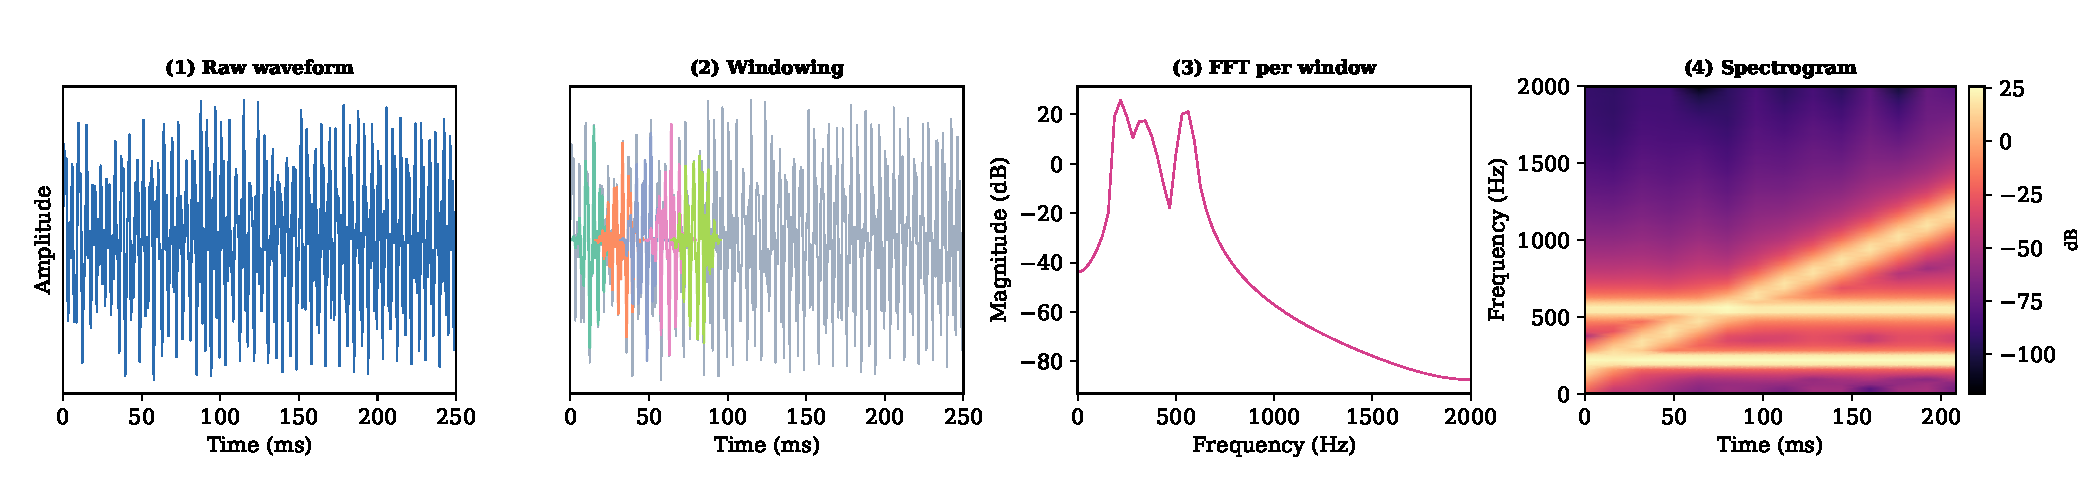
\includegraphics[width=\textwidth]{figures/stft_pipeline.pdf}
    \caption{Audio-to-spectrogram pipeline: raw waveform (time domain), overlapping windowing, FFT on each window, and final time-frequency spectrogram representation.}
% \label{fig:stft_pipeline}
\end{figure}

The choice of window size involves a fundamental trade-off between temporal and frequency resolution. Shorter windows provide better temporal resolution (the ability to pinpoint when a frequency appears) but worse frequency resolution (the ability to distinguish between closely spaced frequencies). Longer windows provide the opposite.  This trade-off is inherent to the uncertainty principle in signal processing and cannot be avoided, only managed according to the requirements of the task\cite{hendrikpurwins20191}.

The spectrogram is a powerful representation because it makes the structure of audio visually apparent: sustained tones appear as horizontal bands, percussive events as vertical lines, and harmonic sounds as stacks of parallel bands at integer multiples of a fundamental frequency.  However, the raw STFT spectrogram has a linear frequency axis, which does not correspond well to how humans perceive pitch.

\subsection{The Mel Scale and Mel Spectrograms}

Human pitch perception is approximately logarithmic: the perceived difference between 100 Hz and 200 Hz is much greater than between 5,000 Hz and 5,100 Hz, even though the absolute difference in Hertz is the same. The mel scale is a perceptual scale of pitch that reflects this nonlinearity. It was derived from psychoacoustic experiments in which listeners were asked to judge equal intervals of pitch, and it maps frequencies so that equal distances on the mel scale correspond to equal perceived pitch intervals.

A mel spectrogram is obtained by projecting the frequency axis of a standard STFT spectrogram onto a set of mel-spaced triangular filter banks. The mel filter bank for projecting frequencies is inspired by the human auditory system and physiological findings on speech perception.\cite{hendrikpurwins20191}  These filters are narrowly spaced at low frequencies (where human frequency discrimination is fine) and more widely spaced at high frequencies (where discrimination is coarser). The magnitudes within each filter band are summed, resulting in a reduced number of frequency bins that better reflect perceptual relevance. Applying a logarithmic transformation to these magnitudes yields the log-mel spectrogram, which further aligns the representation with human loudness perception.

[FIGURE: Linear spectrogram vs. mel spectrogram comparison. Two side-by-side spectrograms of the same audio excerpt: (left) linear frequency axis, (right) mel-scaled frequency axis. Annotate the mel version to show how low frequencies get more resolution than high frequencies. Format: generate in Python with librosa and export as images.]

The log-mel spectrogram has become the dominant input representation for deep learning models applied to audio.\cite{hendrikpurwins20191}  It provides a compact, perceptually motivated summary of the audio signal that retains the information most relevant to human hearing while discarding redundancy in the high-frequency range. Compared to raw waveforms, log-mel spectrograms require significantly less data and training time to achieve comparable classification performance, making them the practical default for most MIR tasks.\cite{hendrikpurwins20191}  

\subsection{Audio Features}

While spectrograms provide a rich, general-purpose representation of audio, many MIR tasks benefit from extracting specific numerical descriptors, called audio features, that capture particular aspects of the signal. These features can be broadly categorized into spectral, temporal, and tonal features.

\textbf{Spectral features} describe the shape and characteristics of the frequency spectrum at a given moment. The spectral centroid represents the center of mass of the spectrum and correlates with the perceptual quality of brightness: sounds with energy concentrated at higher frequencies have a higher spectral centroid. The spectral bandwidth measures the dispersion of energy around the centroid, indicating timbral richness.  Spectral flux quantifies how much the spectrum changes between consecutive frames, making it particularly useful for detecting onsets and transient events in music. The spectral rolloff is the frequency below which a specified percentage (typically 85\% or 95\%) of the spectral energy is concentrated, serving as an indicator of the spectral shape and harmonicity of the sound. The spectral contrast captures the dynamic range between peaks and troughs across frequency sub-bands, providing information about timbral texture. 

\textbf{Mel-Frequency Cepstral Coefficients (MFCCs)} are a compact representation of the spectral envelope. They are computed by taking the discrete cosine transform (DCT) of the log-mel spectrum, which decorrelates the filter bank energies and compresses the information into a small number of coefficients (typically 13 to 20). For decades, MFCCs were the dominant feature representation in audio analysis, particularly in speech recognition.\cite{hendrikpurwins20191}  In the context of deep learning, their use has declined in favor of log-mel spectrograms, since the DCT step that produces MFCCs discards spatial relationships between frequency bands that convolutional neural networks can exploit directly.\cite{hendrikpurwins20191}  Nevertheless, MFCCs remain a standard feature in many MIR pipelines and provide a useful, low-dimensional summary of timbral characteristics.

\textbf{Temporal features} describe properties of the signal in the time domain. The zero-crossing rate (ZCR) measures how frequently the signal changes sign, which correlates with the noisiness or percussive character of the sound.  Root mean square (RMS) energy provides a frame-level measure of loudness. Onset strength functions measure the likelihood of a musical onset (the beginning of a note or percussive hit) at each time step, typically derived from the rate of increase in spectral energy.

\textbf{Tonal and chroma features} capture pitch-class information independently of octave. A chroma feature vector represents the energy distribution across the twelve pitch classes of the Western chromatic scale (C, C\#, D, ..., B), collapsing octave information so that all instances of a given note class contribute to the same bin. Chroma features can be derived from the STFT (Chroma STFT), the Constant-Q Transform (Chroma CQT, which offers better frequency resolution at low frequencies), or computed with energy normalization and temporal smoothing (Chroma CENS) for more robust harmonic pattern recognition.  These features are particularly relevant for tasks involving harmonic analysis, chord recognition, and key estimation.

[FIGURE: Summary of audio features. A diagram or table showing the main feature categories (spectral, cepstral, temporal, tonal) with representative features listed under each, and a brief note on what musical quality each captures (e.g., spectral centroid → brightness, chroma → harmonic content). Format: could be a simple TikZ table or a structured diagram.]

The choice of which features to extract depends on the task at hand. Beat tracking systems typically operate on onset strength functions or spectral flux, while systems concerned with mood or energy may rely more heavily on spectral centroid, loudness curves, and MFCCs. For the system described in this thesis, which must translate audio into lighting parameters that reflect both rhythmic and timbral qualities of the music, a combination of spectral, temporal, and rhythmic features is relevant. The specific feature extraction pipeline is discussed in Chapter 6.

\section{Musical Structure and Beat Tracking}

The previous section established how raw audio can be transformed into feature representations that capture different musical qualities. This section turns to the musical structures those features are ultimately meant to describe: rhythm, meter, and form. It begins with the fundamentals of rhythmic organisation, moves to the specific structural conventions of electronic dance music, and then formalises beat tracking as a computational task.

\subsection{Rhythmic Fundamentals}

Music unfolds as a sequence of events in time, and the most basic organising principle of that temporal flow is the beat: a perceived regular pulse that listeners naturally tap along to. The rate at which beats occur is the tempo, conventionally expressed in beats per minute (BPM). A typical pop or rock track might sit around 100 to 130 BPM, while EDM tempos cluster between roughly 120 and 130 BPM for genres like house and progressive house,  and may reach 140 BPM or higher in trance and drum-and-bass.

Not all beats carry equal perceptual weight. Western music groups beats into recurring patterns of strong and weak pulses called meter. The first beat of each group, the downbeat, is perceived as metrically strongest. The grouping itself defines the time signature: a 4/4 meter groups four beats per measure (or bar), with the downbeat on beat one; a 3/4 meter groups three. These patterns create a metrical hierarchy, a layered grid ranging from sub-beat divisions (such as eighth or sixteenth notes) up through beats, downbeats, and multi-bar phrases. Listeners unconsciously infer this hierarchy from the acoustic signal, and it guides expectations about when the next salient event will occur.

This hierarchical view matters for computational systems because different applications need different levels of the grid. A simple visualiser that flashes on every beat needs only the beat level. A lighting controller that distinguishes verse from chorus needs the downbeat level (to know where measures begin) and, ideally, a sense of higher-level phrasing (to know where sections change). Beat tracking and downbeat tracking are therefore treated as distinct but related tasks in MIR. 

[FIGURE: Metrical hierarchy diagram. Show a four-bar excerpt in 4/4 time as a tree or layered grid: the top row marks the four-bar phrase boundary, the next row marks downbeats (bar lines), the next row marks individual beats, and the bottom row marks sub-beat divisions (eighth notes). Label each level. This can be drawn as a simple TikZ grid or adapted from standard music theory textbooks.]

\subsection{EDM Form and Structure}

Electronic dance music occupies a distinctive position in the landscape of popular music. Its rhythmic foundation is overwhelmingly grid-based: sequences are quantised to exact metric positions, and the dominant rhythmic pattern is the four-on-the-floor kick drum, a bass drum striking on every beat of a 4/4 bar.  Brøvig-Hanssen et al. observe that EDM "literally sound[s] like a machine" by presenting musical patterns that "act like machines, and by cultivating aesthetic qualities that we associate with machines (such as precision [and] speed)."\cite{ragnhildtorvangersolberg20142}  This grid-based precision might seem to leave little room for expressive nuance, yet producers manipulate sonic features such as attack shape, sidechain compression, and swing quantisation to introduce subtle rhythmic friction that makes the groove feel alive rather than mechanical. 

At the macro level, EDM tracks follow a broadly predictable formal scheme. Butler (2006) and Snoman (2009) identify a conventional template in which a track contains two cycles of build-up and drop, with the second cycle typically more intense than the first.\cite{ragnhildtorvangersolberg20142}  Solberg (2014) refines this into a framework centred on three key sections: the breakdown, the build-up, and the drop. These names reflect their musical function. The breakdown strips the track's texture down, removing layers and, crucially, removing the bass and bass drum, the rhythmic foundation on which dancers rely and coordinate themselves. The build-up that follows gives strong indications of a massive musical, emotional, and bodily peak ahead. The drop then reintroduces the bass and bass drum, resolving the accumulated tension in what is often the most intense moment of the track.\cite{ragnhildtorvangersolberg20142}  A complete track typically frames these cycles within an intro and outro that facilitate DJ mixing.

[FIGURE: EDM macro-structure and intensity curve. A horizontal timeline of a typical EDM track divided into labelled sections: Intro, Build-up 1, Drop 1, Breakdown, Build-up 2, Drop 2, Outro. Overlay a smooth intensity or energy curve that dips during breakdowns and peaks at drops. Adapted from the structural scheme described by Butler (2006) and Solberg (2014). This works well as a simple TikZ diagram with a shaded area plot.]

What makes this formal structure audible to listeners (and potentially detectable by computational systems) is a set of production techniques that function as structural markers. Solberg identifies five dominant techniques used in build-ups and drops: (i) extensive use of uplifters, rising noise sweeps or pitched sounds that create a sensation of upward motion; (ii) the "drum roll effect," a rhythmic acceleration of percussive hits as the drop approaches; (iii) large frequency changes, often achieved through filter sweeps; (iv) the removal and reintroduction of the bass and bass drum; and (v) a contrasting breakdown that heightens the impact of the subsequent drop.\cite{ragnhildtorvangersolberg20142}   

Smith (2021) provides a complementary analytical framework by focusing specifically on continuous processes: musical gestures characterised by continuous changes to parameters, as opposed to discrete, step-by-step ones. Examples include pitch slides (glissandos), crescendos, fade-ins, accelerandos, filter sweeps, and timbre changes accomplished through manipulation of sound envelopes and frequency content. These processes are created through continuous controllers such as sliders and knobs, or programmed into tracks with automation curves. Functionally, Smith argues, continuous processes serve three roles. In core sections they provide ornamentation, embellishing rhythms and melodies. In build-up sections they provide orientation, often accompanied by intensification, guiding listeners toward structural boundaries so they can anticipate the drop and coordinate their bodies to the beat. In breakdown sections they can produce disorientation, creating sounds that are hard to interpret within the prevailing meter and tempo, signalling to dancers that they can take a break.\cite{jeremywsmithnd3}   

Together, these structural and production conventions mean that EDM tracks, despite their repetitive surface, contain clear hierarchical organisation at multiple time scales: sub-beat rhythmic patterns, four-on-the-floor metric regularity, multi-bar phrases, and section-level formal structure marked by systematic changes in energy, spectral content, and textural density. This layered organisation is what an automated music analysis system must capture if it is to drive meaningful visual responses.

\subsection{Beat Tracking}

Beat tracking, the task of estimating the temporal locations of musical beats in an audio signal, is one of the long-standing problems in MIR.\cite{francescofoscarinnd4}  It is often combined with downbeat tracking, which targets the higher metrical level of identifying the beginning of each measure.  Both tasks are fundamental to any system that needs to synchronise visual output with music.

Historically, beat tracking grew out of onset detection, the task of identifying starting points of musically relevant events such as notes.  Early onset detectors used hand-designed spectral features like spectral flux to detect sudden changes in the frequency content of a signal. However, modern beat tracking systems tackle the task more directly without relying on a separate onset detection stage.\cite{hendrikpurwins20191}   

Most recent systems follow a common pipeline consisting of three stages. First, the audio is transformed into a time-frequency representation, typically a mel spectrogram. Second, a neural network (often a convolutional recurrent neural network, or CRNN) processes the spectrogram to produce frame-wise beat and downbeat activation values: a probability for each time frame indicating how likely it is to contain a beat or downbeat. Third, a post-processing stage converts these noisy, continuous activations into discrete beat positions.\cite{francescofoscarinnd4}   

[FIGURE: Beat tracking pipeline. A horizontal block diagram showing four stages from left to right: Audio Waveform → Spectrogram (mel spectrogram) → Neural Network (producing beat/downbeat activations as a probability curve) → Post-Processing (producing final beat positions as vertical markers on a timeline). Label each block and show a small illustrative visual inside each: a waveform, a spectrogram image, an activation curve, and evenly-spaced beat markers.]

The most widely used post-processing method is the Dynamic Bayesian Network (DBN) in the form proposed by Böck et al. (2011). The DBN imposes a probabilistic model over tempo and meter, forcing the predicted beats to conform to musically plausible constraints: a tempo range (typically 55 to 215 BPM), a set of allowed time signatures (typically 3/4 and 4/4), and a degree of tempo continuity.\cite{francescofoscarinnd4}   This works well for the majority of popular music, where tempo and meter are stable, but it can fail on pieces that deviate from these assumptions, such as music with tempo changes, unusual time signatures, or rubato performance. An alternative post-processing paradigm is particle filtering, used by systems like BeatNet and its successor BeatNet+. In particle filtering, a set of particles represents and evolves the posterior distribution of rhythmic states (beat, downbeat, non-beat) over time, allowing the system to track tempo changes more flexibly than the DBN.  BeatNet+ combines a CRNN front-end with a two-level cascade Monte Carlo particle filter to perform real-time joint beat, downbeat, and meter tracking.\cite{mojtabaheydari20245}   

A critical distinction for real-time applications is between offline and online beat tracking. Offline systems have access to the entire audio recording and can use bidirectional models and global optimisation, yielding the highest accuracy. Online (or causal) systems must produce beat estimates using only past and present audio frames, which is substantially harder. Recent advances in online tracking include BEAST (Chang and Su, 2024), which applies a streaming Transformer encoder with contextual block processing to produce beat and downbeat activations from partially available audio frames, achieving an F1 score of 80.04\% for beats under a 46-millisecond latency constraint.\cite{chihchengchang20236}   The PLP-based system of Meier et al. (2024) takes a different approach, building on the predominant local pulse concept to achieve zero-latency beat tracking with a lookahead mechanism that can predict beats several hundred milliseconds in advance.\cite{petermeier20247}   At the offline end of the spectrum, Foscarin et al. (2024) demonstrate that a carefully designed neural architecture combining convolutions and transformers can achieve state-of-the-art F1 scores (92.6\% for beats, 85.4\% for downbeats) without any DBN post-processing at all, using instead a minimal peak-picking strategy and a novel "sum head" that ensures downbeat predictions always coincide with beat predictions.\cite{francescofoscarinnd4}   

Beat tracking performance is evaluated using several standard metrics. The F1 score, computed with a tolerance window (typically ±70 milliseconds), measures the proportion of correctly detected beats. Two additional continuity-based metrics, CMLt (Correct Metrical Level, continuity-required) and AMLt (Allowed Metrical Levels, continuity-required), impose a stricter criterion: a beat is counted as correct only if both it and the preceding beat are correctly placed, ensuring that the tracker maintains a consistent pulse rather than producing isolated correct hits. AMLt further allows predictions at alternative metrical levels (such as double or half tempo, or offbeats), accommodating the inherent ambiguity of metrical interpretation.\cite{francescofoscarinnd4}   For a real-time audio-visual system like the one developed in this thesis, the F1 score and latency are the most practically relevant metrics: the system must detect beats accurately and quickly enough for the visual response to feel synchronised with the music.

\section{Deep Learning Architectures for Audio Analysis}

The beat tracking and music analysis systems discussed in the previous section rely on deep neural network architectures that have been adapted from other domains, principally computer vision and natural language processing, to the unique challenges of audio signals. This section provides a theoretical overview of the four principal architecture families used in modern music information retrieval: convolutional neural networks (CNNs), recurrent neural networks (RNNs), convolutional recurrent neural networks (CRNNs), and Transformer-based models. Understanding these building blocks is essential for the chapters that follow, as the system developed in this thesis employs a pipeline that combines several of them.

\subsection{Convolutional Neural Networks}

The connection between audio and convolutional neural networks begins with the spectrogram representation introduced in Section 2.1. Once audio has been converted into a mel spectrogram, the resulting two-dimensional time-frequency matrix can be treated as a single-channel image, making it possible to apply CNNs directly.\cite{hendrikpurwins20191}   A CNN processes its input by sliding small learnable filters (also called kernels) across the input matrix, computing a dot product at each position to produce a feature map that highlights local patterns such as harmonic structures, onset transients, or percussive events.  After each convolutional layer, a non-linear activation function (typically a rectified linear unit, or ReLU) is applied element-wise. Successive convolutional layers build a hierarchy of increasingly abstract features: early layers detect simple edges or frequency bands, while deeper layers combine these into higher-order representations such as timbral textures or rhythmic motifs.

Pooling layers follow convolution to reduce the spatial dimensions of the feature maps, providing a degree of translational invariance and lowering computational cost. Max pooling, which selects the maximum value within a local window, is the most common variant. An alternative to increasing the receptive field through pooling is the use of dilated (atrous) convolutions, which insert gaps between the filter elements so that each layer covers a wider span of the input without increasing the number of parameters.  In MIR, convolutional architectures have been successfully applied to a wide range of tasks, including beat tracking, onset detection, chord recognition, instrument classification, and automatic music tagging.\cite{hendrikpurwins20191}  

\subsection{Recurrent Neural Networks and LSTMs}

While CNNs excel at capturing local spectral and temporal patterns within their receptive field, audio is inherently sequential: the musical significance of a note, chord, or beat depends on the context established by preceding events. Recurrent neural networks (RNNs) address this by maintaining a hidden state vector that is updated at each time step using both the current input and the previous hidden state, creating a form of memory that allows information to propagate from earlier frames to later ones.\cite{hendrikpurwins20191}  

In practice, standard RNNs struggle with long-range dependencies because gradients either vanish (shrink toward zero) or explode (grow unboundedly) during backpropagation through time. The Long Short-Term Memory (LSTM) architecture solves this problem by introducing a gating mechanism. Each LSTM unit contains three gates: an input gate that controls how much new information enters the cell state, a forget gate that controls how much of the existing cell state is retained, and an output gate that controls how much of the cell state is exposed as the unit's hidden output.\cite{hendrikpurwins20191}   Together, these gates allow the LSTM to selectively remember or discard information over hundreds of time steps, making it far more effective than a standard RNN at modelling the kind of long-range temporal structure found in music, from phrase-level patterns to section-level repetitions.

Bidirectional variants (BiLSTMs) process the input sequence in both the forward and backward directions, concatenating the two hidden states at each time step to produce a representation that incorporates both past and future context. BiLSTMs are commonly used in offline MIR tasks where the entire recording is available before processing begins.\cite{hendrikpurwins20191}  

\subsection{Convolutional Recurrent Neural Networks}

The complementary strengths of CNNs and RNNs lead naturally to their combination in convolutional recurrent neural networks (CRNNs). In a CRNN, a stack of convolutional layers first extracts compact, high-level feature vectors from the spectrogram input, and these feature sequences are then passed to one or more recurrent layers (typically LSTMs or GRUs) that model their temporal evolution.  This design separates two distinct modelling responsibilities: the CNN front-end learns what to extract from each spectrogram frame (spectral shape, harmonic content, onset strength), while the RNN back-end learns how these features change over time (tempo regularity, metrical cycles, structural boundaries).\cite{hendrikpurwins20191} 

The CRNN has become the dominant architecture for frame-level music analysis tasks, including beat tracking, onset detection, chord recognition, and vocal melody extraction.\cite{hendrikpurwins20191}   A representative example discussed in Section 2.2 is BeatNet+, whose architecture consists of three convolutional layers followed by four LSTM layers, producing frame-wise beat and downbeat activation functions from a log-frequency spectrogram input.\cite{mojtabaheydari20245}   CRNNs have also been the standard architecture for online (causal) beat tracking systems, where the recurrent component naturally processes audio one frame at a time in a streaming fashion.\cite{chihchengchang20236}   The practical success of the CRNN across so many MIR tasks can be attributed to this clean separation of concerns: convolution handles the local, spatial structure of the spectrogram, while recurrence handles the global, temporal structure of the music.

[FIGURE: Deep learning building blocks for audio analysis. A diagram showing four architecture families as increasingly complex assemblies: (1) a CNN block consisting of convolutional layers with pooling operating on a spectrogram, (2) an RNN/LSTM block showing recurrent connections across a sequence of time steps, (3) a CRNN that combines both by feeding CNN output into an RNN, and (4) a Transformer block built from multi-head self-attention and position-wise feed-forward layers. Arrows indicate how each architecture builds on or extends the previous one. Adapted from Purwins et al. (2019), Figure 2.]

\subsection{Attention and the Transformer Architecture}

Despite their effectiveness, recurrent networks process sequences one step at a time, creating a computational bottleneck and making it difficult to capture dependencies between distant time steps efficiently. The attention mechanism addresses this limitation by allowing the network to compute a weighted combination of all positions in a sequence when producing the representation for any single position, effectively bypassing the sequential processing constraint.\cite{hendrikpurwins20191}   Rather than compressing an entire history into a single fixed-size hidden state, attention lets the model look back at all previous (or all surrounding) time steps and assign a learned relevance weight to each, so that the most informative positions contribute most to the current output.

The Transformer architecture, introduced by Vaswani et al. (2017),\cite{vaswani2023attentionneed}  builds entirely on self-attention and dispenses with recurrence altogether. In each Transformer layer, multi-head self-attention computes several parallel attention functions, each learning to attend to different aspects of the input relationships (for instance, one head might attend to rhythmic periodicity while another captures harmonic similarity). This is followed by a position-wise feed-forward network, with residual connections and layer normalisation stabilising training. Because the Transformer has no inherent notion of sequential order, explicit positional encodings must be added to the input to provide information about the position of each element in the sequence. Since all positions are processed in parallel rather than sequentially, Transformers are both faster to train on modern GPU hardware and more effective at modelling long-range dependencies than RNNs, though their memory and computation scale quadratically with sequence length.

The adoption of Transformers in MIR is relatively recent but rapidly growing. BEAST (Chang and Su, 2024) was the first system to apply a streaming Transformer to online beat and downbeat tracking, replacing the recurrent layers of the traditional CRNN pipeline with a Transformer encoder that uses contextual block processing.\cite{chihchengchang20236}   To handle the streaming (causal) constraint, BEAST employs relative positional encodings inspired by Transformer-XL, which allow the model to attend to a bounded window of past context without requiring access to the full recording.\cite{chihchengchang20236}   At the offline end of the spectrum, the "Beat this!" system of Foscarin et al. (2024) combines a convolutional front-end with a Transformer backbone consisting of six encoder blocks using rotary positional embeddings, demonstrating that a convolution-plus-Transformer design can achieve state-of-the-art beat tracking accuracy without any recurrence-based post-processing.\cite{francescofoscarinnd4}    These systems illustrate a broader pattern in which Transformers are not replacing CNNs entirely but rather replacing the recurrent component of CRNNs, yielding hybrid convolution-Transformer architectures that combine the local feature extraction of convolutions with the global context modelling of self-attention.

Beyond single-task classification, the Transformer architecture also supports encoder-decoder configurations for sequence-to-sequence tasks, where one sequence (such as a musical audio representation) is mapped to a different output sequence (such as a lighting control sequence). The BART (Bidirectional and Auto-Regressive Transformers) architecture exemplifies this design: it combines a bidirectional Transformer encoder, which reads the entire input in full context, with an autoregressive Transformer decoder, which generates the output sequence one token at a time.\cite{zijianzhao202510}   BART is pre-trained using a denoising objective in which the input is corrupted (for example, by masking spans of tokens) and the model learns to reconstruct the original, giving the encoder a deep understanding of the input structure.\cite{zijianzhao202510}   This encoder-decoder formulation is central to the Skip-BART model used in this thesis and is examined in detail in the following section.

The progression from CNNs through CRNNs to Transformers reflects a broader trend in deep learning for audio: each successive architecture captures increasingly global temporal context while reducing or eliminating the sequential bottleneck inherent in recurrence. The system developed in this thesis draws on multiple points along this progression. The beat tracking component relies on CRNN and Transformer-based architectures as discussed in Section 2.2, while the lighting generation component uses the BART encoder-decoder architecture, whose sequence-to-sequence formulation is the subject of Section 2.4.

\section{Sequence-to-Sequence Models and the BART Architecture}

The previous section surveyed the deep learning building blocks used for audio analysis: CNNs for local spectral pattern extraction, RNNs for temporal modelling, CRNNs that combine both, and Transformers that replace recurrence with self-attention. The present section narrows the focus to one particular configuration of the Transformer that is central to the lighting generation component of this thesis: the encoder-decoder, or sequence-to-sequence, architecture, and its instantiation in BART.

\subsection{The Sequence-to-Sequence Framework}

Many audio processing tasks are essentially sequence-to-sequence transduction tasks, in which an input sequence of one modality or representation must be mapped to an output sequence of potentially different length or modality. A sequence-to-sequence model transduces an input sequence into an output sequence directly, without requiring the two sequences to be the same length or to share a common vocabulary. The paradigm emerged from neural machine translation, where the goal is to map a sentence in one language to a sentence in another, but it has since been adopted for speech recognition, music transcription, and, as this thesis demonstrates, cross-modal generation tasks such as mapping music to lighting.

In the formulation described by Purwins et al. (2019), the context at each decoder step is a weighted sum of the encoder embeddings, where the weights are calculated between the current decoder embedding and all encoder embeddings, indicating correlations between input and output positions.\cite{hendrikpurwins20191}  With the adoption of RNNs for sequence modelling, the research field shifted towards these full sequence-to-sequence models, and despite their architectural simplicity, further improvements in both model structure and optimisation process have been proposed.\cite{hendrikpurwins20191} 

The Transformer architecture, discussed in Section 2.3, replaced the recurrent components of the encoder and decoder with self-attention layers, yielding a fully attention-based sequence-to-sequence model. This Transformer-based encoder-decoder design forms the backbone of the architecture discussed next.

\subsection{Denoising Pre-training and the BART Architecture}

BART (Bidirectional and Auto-Regressive Transformers), introduced by Lewis (2019),\cite{lewis2019bartdenoisingsequencetosequencepretraining}  combines a bidirectional Transformer encoder with an autoregressive Transformer decoder.\cite{zijianzhao202510}  The encoder reads the entire input sequence with full bidirectional attention, building a rich contextual representation of every position. The decoder then generates the output sequence left-to-right, attending to the encoder's representations through cross-attention and to its own previously generated tokens through causal (masked) self-attention.

What distinguishes BART from encoder-only models such as BERT or decoder-only models such as GPT is that it is pre-trained using a denoising objective: the input text is corrupted by applying one or more noise functions (such as token masking, token deletion, sentence permutation, or span infilling), and the model is trained to reconstruct the original, uncorrupted text.\cite{lewis2019bartdenoisingsequencetosequencepretraining}  This pre-training strategy forces the encoder to develop a deep understanding of the input structure while training the decoder to generate fluent, coherent output, making BART particularly effective for generation tasks.

The BART architecture has been successfully adapted beyond natural language. PianoBART (Liang et al., 2024) applies the same framework to symbolic music, pre-training on large-scale piano MIDI data to learn latent musical representations and then fine-tuning on downstream tasks such as melody extraction and emotion classification.\cite{zijianzhao202510}  As discussed below, the Skip-BART model developed by Zhao et al. (2025) extends this cross-domain adaptation further, from symbolic music to a cross-modal setting in which the encoder processes audio representations and the decoder generates lighting control sequences.\cite{zijianzhao202510} 

[FIGURE: The BART encoder-decoder architecture. On the left, the bidirectional encoder processes a corrupted input sequence (with some tokens masked or deleted). On the right, the autoregressive decoder reconstructs the original sequence, attending to the encoder's output through cross-attention at each layer. Show the flow of information: input tokens → encoder layers (bidirectional self-attention) → cross-attention → decoder layers (causal self-attention) → output tokens. Adapted from Lewis (2019) and the Skip-BART paper's Figure 1.]

\subsection{Cross-Modal Adaptation}

The application of BART to automated stage lighting control (ASLC) requires bridging two fundamentally different modalities: continuous audio representations on the encoder side and discrete lighting parameters on the decoder side. Zhao et al. (2025) frame ASLC as a generative task rather than a rule-driven mapping process, arguing that lighting design is essentially an art creation process and proposing the first end-to-end deep learning method for stage lighting generation.\cite{zijianzhao202510}\cite{zijianzhao202510} 

On the encoder side, the music input is represented using OpenL3 (Cramer et al., 2019), a deep neural network architecture that extracts high-level auditory embeddings through audio-visual correspondence learning.\cite{zijianzhao202510}  These continuous embeddings are passed through an MLP to align their dimensionality with the BART backbone before being fed into the encoder.\cite{zijianzhao202510} 

On the decoder side, the lighting output is represented in the HSV colour space (discussed in detail in Section 2.5), with the Saturation channel fixed at maximum and only the Hue (H) and Value (V) channels modelled. Rather than treating these as continuous values, Skip-BART tokenises them into discrete categories: hue values range from 0 to 179 and value (brightness) levels from 0 to 255, yielding vocabulary sizes of 180 and 256 respectively.\cite{zijianzhao202510}  This tokenisation approach is essential because directly processing hue data with an MLP presents challenges due to the cyclical nature of hue values: the minimum and maximum hue values can be quite similar, complicating the learning process; in contrast, the embedding layer effectively captures the relationships between different tokens, making it more suitable for handling cyclic data like hue.\cite{zijianzhao202510}  The tokenised hue for each frame is computed as the mode of the hue distribution, while the tokenised value is computed as the weighted average of the value distribution.\cite{zijianzhao202510} 

A distinctive architectural contribution of Skip-BART is its skip connection mechanism. When applying BART for the lighting generation task, the attention mechanism in the decoder struggles to determine which light frame corresponds to which music frame, even though the music input and light output have the same temporal length. To address this, the skip mechanism directly combines the music embedding and light embedding before inputting them to the decoder, explicitly indicating the one-to-one correspondence between music frames and light frames. This is particularly important because the model must learn this frame-level alignment from complex and noisy data in an end-to-end manner.\cite{zijianzhao202510} 

The backbone of Skip-BART directly incorporates pre-trained parameters from PianoBART, providing a solid starting point for subsequent training through cross-modal transfer learning.\cite{zijianzhao202510}  To combine knowledge from PianoBART's multiple downstream tasks (melody extraction, velocity prediction, composer classification, and emotion classification), the Drop And Rescale (DARE) method (Yu et al., 2024) is used to merge the fine-tuned parameters,\cite{zijianzhao202510}  and LoRA (Low-Rank Adaptation; Hu et al., 2022) is employed for efficient tuning, keeping the majority of backbone parameters frozen.\cite{zijianzhao202510} 

\subsection{Parameter-Efficient Fine-Tuning and Inference}

The combination of transfer learning, DARE merging, and LoRA results in a model with approximately 240 million total parameters but only 19 million trainable parameters.\cite{zijianzhao202510}  This parameter efficiency is critical given the limited size of stage lighting datasets.

[FIGURE: Skip-BART workflow diagram showing the three phases: (1) Pre-training, where the encoder processes masked music sequences and the decoder reconstructs them using a BART-based masked language modelling objective with a discriminator; (2) Fine-tuning, where the encoder receives music embeddings from OpenL3 and the decoder is trained to predict discrete hue and value tokens using a classification head; (3) Inference, where the decoder generates lighting tokens autoregressively using RSTC sampling. Adapted from Zhao et al. (2025), Figure 3.]

The model is pre-trained using a BART-based masked language modelling approach. During pre-training, only the music data is used (without light) to avoid information leakage. The encoder encodes the masked music sequence, while the decoder receives the shift-right ground truth as input and attempts to recover the original music sequence. Although there is a gap between the music modality in pre-training and the light modality in fine-tuning, this approach has been demonstrated to be effective, supported by the theory of cross-modal transfer learning.\cite{zijianzhao202510}  During fine-tuning, the model is trained end-to-end to generate the corresponding lighting sequences using a next-token prediction objective framed as a classification task over the hue and value vocabularies.\cite{zijianzhao202510} 

During inference, Skip-BART generates the lighting sequence in an autoregressive manner, producing one lighting token at a time conditioned on the full music input and all previously generated tokens.\cite{zijianzhao202510}  To prevent model degradation while maintaining diversity, a stochastic temperature-controlled sampling method is employed, in which the temperature parameter controls the randomness of the sampling distribution.\cite{zijianzhao202510}  Additionally, to avoid abrupt changes in the generated lighting, a restriction mechanism ensures that successive lighting tokens do not exceed a specified threshold in hue or value distance.\cite{zijianzhao202510}  This combined approach is termed Restricted Stochastic Temperature-Controlled (RSTC) sampling: the probability of all categories exceeding the distance threshold is set to zero during sampling, ensuring both diversity and temporal smoothness in the generated output.\cite{zijianzhao202510} 

The theoretical concepts introduced in this section, particularly the encoder-decoder architecture, the denoising pre-training paradigm, and the cross-modal adaptation strategies, provide the foundation for understanding how the system developed in this thesis generates lighting from audio input. The next section examines the perceptual and aesthetic principles that inform what kind of lighting the system should produce.

\section{Stage Lighting and Music-Visual Mapping}

The previous sections have established the computational and architectural foundations of the system: how audio is represented and analysed (Section 2.1), how musical structure is defined and detected (Section 2.2), which deep learning architectures process audio signals (Section 2.3), and how the BART encoder-decoder generates output sequences from input sequences (Section 2.4). This section turns to the output side of the pipeline: stage lighting. It examines the colour model used to represent lighting states, the perceptual and psychological evidence for systematic associations between music and colour, and the evolution of automated stage lighting control from rule-based approaches to the generative paradigm adopted in this thesis.

\subsection{The HSV Colour Model}

Stage lighting is most naturally described in terms of colour and brightness rather than the red-green-blue (RGB) channel decomposition used internally by display hardware. The HSV (Hue, Saturation, Value) colour space provides exactly this separation. Hue encodes the colour itself as an angle on a colour wheel, Saturation encodes the purity or vividness of the colour, and Value encodes its brightness. This decomposition makes the control and generation of lighting more intuitive, independent, and stable, because a lighting designer (or a generative model) can adjust brightness without affecting colour, or shift colour without changing intensity.\cite{zijianzhao202510} 

In the implementation used by Zhao et al. (2025) for the Skip-BART model, the HSV representation is applied following the OpenCV convention. The Hue channel ranges from 0 to 179, representing 180 discrete hue categories on a cyclic scale (where 0 and 179 are adjacent, both corresponding to red). The Value channel ranges from 0 to 255, representing 256 brightness levels from completely dark to maximum intensity. The Saturation channel is fixed at 255 (100\%) to simulate vivid stage lighting and counteract environmental influences such as air scattering, fog, or surface reflections that reduce colour purity. This simplification reduces the lighting control problem to two channels, hue and value, while preserving the perceptually most important dimensions for stage lighting design.\cite{zijianzhao202510} 

The cyclic nature of the hue channel presents a specific modelling challenge: the values 0 and 179 are numerically distant but perceptually adjacent (both are red). As discussed in Section 2.4, this is why Skip-BART uses a discrete tokenisation and embedding approach rather than treating hue as a continuous value, since an embedding layer can learn the circular topology that a standard regression head cannot.\cite{zijianzhao202510} 

\subsection{Music-Colour Associations and Emotional Mediation}

The decision to generate coloured lighting from music rests on the assumption that there are systematic, non-arbitrary associations between musical qualities and colours. Experimental evidence supports this assumption. Palmer et al. (2013) conducted a series of experiments in which non-synesthetic participants from the United States and Mexico were asked to choose colours that were most and least consistent with 18 selections of classical orchestral music by Bach, Mozart, and Brahms.\cite{stephenepalmer201313}  The musical selections varied systematically in tempo (slow, medium, fast), mode (major, minor), and composer.

The results revealed robust cross-modal associations between specific musical dimensions and specific colour dimensions. Faster music in the major mode was generally associated with more saturated, lighter, and yellower colours, whereas slower music in the minor mode was associated with more desaturated (greyer), darker, and bluer colours. Critically, these associations were strongly consistent across both the US and Mexican participant groups, suggesting a high degree of cultural invariance.\cite{stephenepalmer201313} 

To explain these associations, Palmer et al. propose the emotional mediation hypothesis: listeners experience an emotional response to the music, and then select colours whose emotional connotations match that response.\cite{stephenepalmer201313}  Separate multidimensional scaling (MDS) analyses of the emotional associations of colours and of musical selections revealed that both could be well explained by the same two emotional dimensions: happy/sad (positive/negative valence) and strong/weak (high/low potency). The correlations between the emotional ratings for the musical selections and the emotional ratings for the colours chosen to go with them were remarkably high: +0.97 for happy/sad, +0.99 for strong/weak, +0.96 for lively/dreary, and +0.89 for angry/calm.\cite{stephenepalmer201313}  Two additional experiments, one mapping colours to emotional facial expressions and another mapping music to emotional faces, provided further converging evidence for the emotional mediation account.\cite{stephenepalmer201313} 

These music-colour associations are distinct from synesthesia. While a small minority of individuals report involuntary cross-modal experiences of colour while hearing musical sounds, scientific studies initially failed to establish general correspondences because synesthetic sound-to-colour mappings appeared idiosyncratic.\cite{stephenepalmer201313}  The associations reported by Palmer et al. are, by contrast, widely shared across non-synesthetic populations. Separately, non-synesthetic people also exhibit relatively low-level auditory-visual associations: higher pitches tend to be associated with lighter colours, and there is evidence for other correspondences such as timbre-saturation, loudness-brightness, and pitch-size associations. Spence (2011) argues that three types of cross-modal matching mechanisms have been established empirically: structural correspondences based on common neural coding, statistical correspondences based on natural covariation of cross-modal attributes, and semantically mediated correspondences based on common descriptive terminology.\cite{stephenepalmer201313}  Palmer et al.'s results provide clear evidence for a fourth type: cross-modal correspondences based on common emotional associations.\cite{stephenepalmer201313} 

[FIGURE: Music-colour association diagram. Show Palmer et al.'s (2013) core finding: a two-panel layout with (left) the emotional space showing how musical selections and colour choices cluster along happy/sad and strong/weak dimensions, and (right) example associations (fast major music → saturated warm colours; slow minor music → desaturated cool colours). Include the key correlation values. Adapted from Palmer et al. (2013).]

For the system developed in this thesis, the emotional mediation framework provides a principled theoretical basis for why music-driven lighting should produce perceptually meaningful results. If listeners consistently associate certain musical qualities with certain colours via shared emotional connotations, then a model trained on real lighting data created by professional lighting engineers should, in principle, learn to reproduce these associations, even without an explicit emotion classification stage.

\subsection{Automated Stage Lighting Control}

Automatic Stage Lighting Control (ASLC) refers to the computational task of generating lighting parameters from music, and it shows potential in live performances by shaping the atmosphere and influencing the emotions of both musicians and audiences, while offering an affordable alternative to human lighting engineers. Although ASLC is not a widely explored topic in MIR, it has received attention in several prior works.\cite{zijianzhao202510} 

Most prior methods follow a two-stage paradigm that first classifies music into predefined categories, such as emotion or style, and then defines a corresponding light pattern for each category.\cite{zijianzhao202510}  Style-based approaches (Stanescu et al., 2018; Lei et al., 2021) and emotion-based approaches (Hsiao et al., 2017; Moon et al., 2015) represent the two mainstream classification strategies.\cite{zijianzhao202510}  Emotion classification methods have employed various machine learning techniques, including Support Vector Machines, Support Vector Regression, and Multi-Layer Perceptrons.\cite{zijianzhao202510}  For the light mapping stage, Hsiao et al. (2017) map music to emotional categories and infer specific lighting patterns based on embeddings in emotional space, while Nijdam (2009) provides a mapping that takes into account both hue and value.\cite{zijianzhao202510}  Other approaches classify music using lyrics (Liao et al., 2023) or chords (Mabpa et al., 2021).\cite{zijianzhao202510} 

These rule-based methods exhibit significant limitations. First, coarse-grained classification severely impacts model performance: categories are typically too broad to capture the nuance of real lighting design.\cite{zijianzhao202510}  Second, there is insufficient theoretical support for deterministically mapping these categories to specific light patterns, since lighting is an amalgam of technology and art rather than a deterministic function.\cite{zijianzhao202510}  Third, the performance of all rule-based methods depends on the accuracy of the upstream classifier, and emotion classification accuracies in many studies fall below 80\%, raising doubts about the practicality of these methods at their current stage.\cite{zijianzhao202510}  Furthermore, many pieces of music lack lyrics or contain lyrics that are difficult to recognise (such as screaming in heavy music), rendering lyrics-based methods ineffective for large portions of the musical repertoire.\cite{zijianzhao202510} 

Zhao et al. (2025) propose a fundamentally different approach by treating ASLC as a generative task.\cite{zijianzhao202510}  Rather than classifying music and then applying predefined mappings, Skip-BART is trained end-to-end on data from professional lighting engineers, learning to generate lighting sequences directly from music in a single pass.\cite{zijianzhao202510}  This generative framing avoids the information bottleneck inherent in classification-based pipelines and allows the model to learn the full complexity and artistry of professional lighting design. Through both quantitative analysis and human evaluation, Skip-BART demonstrates performance closely matching that of real human lighting engineers while significantly outperforming conventional rule-based methods across all evaluation metrics.\cite{zijianzhao202510} 

The theoretical foundations presented in this chapter, from digital audio representation and musical structure through deep learning architectures and the BART sequence-to-sequence framework to the perceptual basis of music-colour associations and the evolution of automated lighting control, collectively provide the knowledge base required to understand the system developed in this thesis. The next chapter builds on this foundation by reviewing related work in greater detail, positioning the contributions of this thesis within the broader research landscape.

\section{Real-Time Audio Processing}

The system described in this thesis must analyse audio and generate lighting responses while music is playing, not after it has finished. This requirement places the system within a class of audio applications that operate under real-time constraints, where the speed of processing is not merely a convenience but a functional necessity. This section defines what real-time operation means in the context of audio processing, examines the sources of latency that constrain system design, and considers the implications of these constraints for the present work.

\subsection{Streaming, Block Processing, and Causality}

Audio algorithms designed for real-time interaction cannot wait for an entire input signal before producing output. Instead, they must process sequential blocks of one or more audio samples at a time, an approach known as block processing or streaming. In generative or analytical models built from multiple neural network layers, every layer must support this scheme: each layer is required to keep track of its internal state between subsequent forward passes to guarantee a continuous output signal between blocks.\cite{francocaspe202514}  For convolutional layers, this is typically achieved through a cached padding mechanism in which the end of the input tensor is retained and used to pad the next input.

A central distinction in streaming systems is between causal and non-causal processing. The outputs of causal systems depend only on current and past inputs, which is a strict requirement for truly real-time streaming models. Non-causal systems, by contrast, incorporate a finite number of future input timesteps, a lookahead, that improves reconstruction or prediction quality at the cost of additional delay. Non-causal models can be reconfigured for causal operation by introducing delays that allow the required future samples to be acquired before processing, but this conversion comes at a latency cost. Although non-causal models typically afford better reconstruction quality, in latency-sensitive applications it is desirable to avoid this additional cumulative delay by training in a causal manner from the outset.\cite{francocaspe202514} 

\subsection{Real-Time Factor}

The standard metric for assessing whether an algorithm can operate in real time is the Real-Time Factor (RTF), defined as the ratio between processing time and the duration of the input: RTF = ${t_p}$/${t_i}$ (${t_p}$ is the processing time and ${t_i}$ is the input time).\cite{francocaspe202514}  An RTF below 1 means the algorithm processes audio faster than it arrives, which is the minimum condition for real-time operation. However, an RTF just below 1 may still be insufficient in practice: low-latency models must process very short audio blocks at a high rate, which severely limits the available computation time for a single inference pass.\cite{francocaspe202514} 

RTF alone does not fully characterise suitability for live use. The Lyria Team at Google DeepMind distinguish live music models from merely fast offline ones by requiring three attributes simultaneously: real-time throughput (RTF $\geq$ 1x), causal streaming in which audio is generated continuously as a function of both user control inputs and past audio output, and responsive controls where the delay between input and output is low enough to facilitate live interaction.\cite{lyriateamnd15}  This tripartite definition is instructive because it highlights that speed (RTF) is a necessary but not sufficient condition for real-time interaction; the processing must also be causal and the end-to-end delay must be perceptually acceptable.

[FIGURE: A diagram illustrating the difference between offline batch processing (entire signal processed at once) and real-time streaming (sequential block processing with causal constraints). Show the input audio being divided into blocks, each processed independently with state carried forward.]

\subsection{Sources of Latency}

Achieving an acceptable RTF does not guarantee low latency. Caspe et al. (2025) present a systematic taxonomy of five architectural sources of latency in interactive audio-to-audio neural systems, providing a useful framework for understanding how delay accumulates in real-time audio processing pipelines.\cite{francocaspe202514} 

Buffering delay arises from the double-buffering approach common to real-time audio systems, in which one audio block is computed while the next is being captured. The total output buffering latency is therefore two block lengths: one for sample acquisition and one for computing.\cite{francocaspe202514}  The block size therefore sets a hard floor on latency and simultaneously determines the upper limit for computation time per block.

Cumulative delay arises when non-causal convolutional layers are reconfigured for streaming by adding a delay line that allows the layers to look ahead in time. This lag accumulates through successive layers and can increase latency in non-causally trained models by hundreds of milliseconds compared to the same architecture trained causally.\cite{francocaspe202514} 

Representation delay refers to the number of samples required for a feature extractor to produce its expected output. Audio models commonly use feature representations such as Pseudo-Quadrature Mirror Filters (PQMF), Short-Time Fourier Transforms (STFT), or Mel filterbanks, each of which introduces its own processing delay.\cite{francocaspe202514}  Linear-phase Finite Impulse Response filterbanks, for instance, exhibit a group delay of approximately half the filter length.

Data-dependent latency is a less widely recognised source. Convolutional layers are effectively FIR filters whose coefficients are learned through training. Models based on convolutional networks can therefore exhibit different degrees of latency depending on the learned coefficients, which are ultimately shaped by the training data. Caspe et al. empirically observed that signals with strong transients, such as percussive drum recordings, resulted in models that prioritised temporal accuracy, yielding lower latency and jitter compared to models trained on sustained harmonic content.\cite{francocaspe202514} 

Finally, positional uncertainty, or jitter, arises from lossy representations computed using block processing. Because the exact position in samples of an event is lost within a block, the model's response depends not only on the input and training method but also on the relative position of the event within a block, introducing a temporal uncertainty of up to one block size.

\subsection{Latency Thresholds and Perceptual Constraints}

The acceptable level of latency depends on the application. For instrumental musical interaction, where a performer's action must produce an audible response that feels immediate, the constraints are particularly strict. Wessel and Wright suggest an upper bound on latency of 10 ms and a jitter of ±1 ms for musical interaction. Empirical studies have supported this recommendation, demonstrating that 10 ms of latency was acceptable to performers in the absence of jitter, while 20 ms of latency or 10 ± 3 ms with jitter significantly degraded the performance experience. The sensitivity of musicians to latency also varies by instrument and monitoring setup, reinforcing the context-dependent nature of this threshold.\cite{francocaspe202514} 

Not all real-time audio applications require instrumental-grade latency, however. Spoken dialogue systems, for example, operate at considerably higher latencies: the Moshi framework uses causal models to encode and decode audio frames of 80 ms, yielding a final latency of 200 ms, which is tolerable for conversational interaction but far above the instrumental threshold.\cite{francocaspe202514}  This range illustrates the principle that latency requirements are fundamentally shaped by the perceptual expectations of the interaction: the tighter the feedback loop between action and response, the lower the tolerable delay.

\subsection{Latency Budgets and Design Trade-offs}

In practice, the total latency of a real-time system is the sum of contributions from each stage in its processing pipeline. Understanding how latency accumulates is therefore essential for system design. Caspe et al. (2025) illustrate this through a detailed analysis of the RAVE neural audio synthesis architecture, revealing how design choices that prioritise reconstruction quality can make a system unsuitable for low-latency interaction. In RAVE's default configuration, the buffering delay alone accounts for 92.9 ms (two blocks of 2048 samples at 44.1 kHz), representation delay from the PQMF filterbank adds 12 ms, and the encoder's high compression ratio of 2048 introduces a jitter span of ±23.2 ms.\cite{francocaspe202514}  When non-causal streaming is enabled, the cumulative delay adds a further 566 ms.\cite{francocaspe202514}  The very features that make RAVE attractive for automatic music generation, namely its high compression ratio and non-causal mode of operation, make it highly unsuitable for low-latency interaction.

The RAVE case study demonstrates that latency reduction requires addressing each source individually and accepting the associated trade-offs. By progressively halving RAVE's compression ratio down to 128 and training causally, Caspe et al. achieved a buffering delay of 5.8 ms with a jitter of ±2.9 ms, approaching their target of 10 ± 1 ms for instrumental interaction.\cite{francocaspe202514}  The broader lesson is that designing for low latency requires putting this issue at the centre of the design problem, carefully inspecting audio representations and architecture to ensure they do not introduce unnecessary delay.\cite{francocaspe202514} 

\subsection{Implications for the Present System}

The latency constraints facing the system developed in this thesis differ from those of instrumental interaction but remain non-trivial. The system does not close an action-to-sound loop in the sense of a digital musical instrument; rather, it analyses incoming audio and produces a visual (lighting) response. Caspe et al. draw a useful distinction between action-to-sound latency, the delay between a performer's gesture and the resulting sound, and sound-to-sound latency, the delay between a captured audio input and the system's output.\cite{francocaspe202514}  The present system operates in a sound-to-light paradigm, where the perceptual tolerance for delay is more generous than for instrumental control but still bounded by the audience's expectation that lighting changes should appear synchronised with musical events.

The total latency budget of the system is the sum of its processing stages: audio capture and buffering, feature extraction (including beat tracking and onset detection), the Skip-BART model's inference for colour prediction, and the rendering of the visual output. Each of these stages contributes its own delay. Beat tracking algorithms, for instance, introduce latency determined primarily by the hop size of their feature extraction and, in the case of transformer-based models, by the look-ahead window. The BEAST streaming beat tracker reports an algorithmic latency of 46 ms at its lowest setting (with a single look-ahead frame), achieving an RTF of 0.41, while the BeatNet system operates at 20 ms latency with an RTF of 0.05.\cite{chihchengchang20236}  The latency of these models is defined as the hop size of the STFT used for feature extraction. There is a direct trade-off between latency and accuracy: BEAST-16, with a 743 ms look-ahead, achieves over 9\% relative improvement in beat F1-score compared to the lowest-latency configuration,\cite{chihchengchang20236}  but at a delay that would be perceptible as a lack of synchronisation between audio and visual events.

The challenge, then, is to select components and configurations that keep the total pipeline latency within a perceptually acceptable range, on the order of tens of milliseconds rather than hundreds, while maintaining sufficient accuracy in the extracted musical features. This is not a matter of optimising a single component but of understanding how latency accumulates across the entire processing chain and making informed trade-offs at each stage. The theoretical framework presented in this section, particularly the latency taxonomy and the distinction between causal and non-causal processing, provides the analytical tools needed to reason about these design decisions in the system implementation described in later chapters.
\chapter{Technology Selection and Platform Constraints}
\label{chap:technologies-and-platform-constraints}

This chapter evaluates the technology, framework, and deployment decisions that define the platform for the prototype, rather than presenting the complete final system design. It is organised by system layer: rendering and 3D graphics, audio capture and processing, machine learning deployment, and frontend application architecture. For each layer, the selected tools are presented, alternatives are compared, and the rationale for selection is justified. The chapter concludes by deriving the platform constraints these decisions impose, which establish the design space developed methodologically and architecturally in Chapter 4.

\section{The Web as a Platform for Real-Time Audio-Visual Applications}

The decision to build this system as a web application is motivated by three considerations: accessibility, portability, and the maturity of the modern browser as an application runtime. A web application requires no installation, runs in any modern browser regardless of operating system, and can be shared with collaborators or evaluators by distributing a URL rather than a platform-specific binary. For a research prototype intended to demonstrate feasibility, this low barrier to entry is a meaningful advantage.

These benefits depend on the browser providing the capabilities required for real-time audio-visual processing. The modern browser exposes the necessary APIs: WebGL for hardware-accelerated 3D rendering, the Web Audio API for low-latency audio capture and spectral analysis, WebAssembly for near-native computational performance, and Web Workers for background-thread execution. Collectively, these APIs make interactive audio-visual applications viable within the browser sandbox.

Alternative approaches were considered. A native C++/OpenGL application would offer unrestricted GPU access and lower audio latency, but would require platform-specific builds and significantly more complex distribution. Electron inherits the browser's resource overhead while losing the zero-install advantage. Game engines such as Unity or Unreal Engine provide powerful rendering and audio capabilities, but introduce a heavy runtime and licensing considerations disproportionate for a stage-lighting research prototype. The web platform, complemented by a local server for ML inference (Section 3.4), provides the best balance of accessibility, development speed, and technical capability for this project.

\section{3D Rendering: WebGL and Three.js}

The visual core of this application is a real-time 3D rendering of a virtual stage with lighting fixtures. WebGL provides the browser's interface to the GPU: a JavaScript API based on OpenGL ES 2.0 that exposes a programmable rendering pipeline without plugins \cite{threejs-docs}. However, WebGL operates at a low level of abstraction, requiring manual management of vertex buffers, GLSL shader programs, and the rendering state machine, which makes it impractical for application-level development.

Three.js addresses this by providing a high-level, scene-graph-based abstraction over WebGL. As the dominant web 3D library \cite{threejs-github,npm-three}, it provides the building blocks this project requires: scene and camera management, a renderer, and a hierarchy of meshes, materials, and lights. Most relevant to this project is the SpotLight primitive, which exposes parameters for colour, intensity, cone angle, penumbra, distance, decay, and target direction. These map directly to the physical characteristics of stage lighting fixtures (PAR cans, moving heads), making SpotLight a natural abstraction for the virtual stage \cite{threejs-docs}. Three.js also supports shadow mapping, post-processing pipelines (bloom, colour grading), and fog simulation, providing the visual vocabulary needed for a convincing stage environment.

The principal alternative, Babylon.js, offers a more comprehensive feature set (built-in physics, visual editor, native WebXR) but produces significantly larger bundles, often exceeding 1 MB even with tree-shaking \cite{babylonjs-forum-bundle-size}, compared to Three.js's approximately 155 KB gzipped \cite{bundlephobia-three}. Since this project requires only lighting, camera controls, and scene composition, Three.js's lighter footprint, larger community, and mature React integration (Section 3.5) make it the better fit.

WebGPU, a next-generation API superseding WebGL, has reached production readiness across all major browsers as of late 2025 \cite{webdev-webgpu-major-browsers-2025,gpuweb-implementation-status}. Three.js already supports a WebGPU renderer alongside its WebGL renderer, so choosing Three.js preserves a clear upgrade path without requiring architectural changes. This project targets the WebGL renderer for maximum compatibility.

\begin{figure}[htbp]
    \centering
    \includegraphics[width=\textwidth]{figures/chapters/3/threejs_scene_graph_and_lighting_model.pdf}
    \caption{Three.js scene graph and lighting model used in this project. The diagram shows a \texttt{Scene} hierarchy with \texttt{PerspectiveCamera}, lighting nodes (\texttt{SpotLight}, \texttt{PointLight}, and \texttt{SpotTarget}), mesh groups for stage elements, and the \texttt{WebGLRenderer} consuming both scene and camera inputs to produce the rendered frame. SpotLight parameters correspond to stage-lighting controls: colour (hue), intensity (value), angle (beam width), penumbra (edge softness), and target (direction).}
\end{figure}

\section{Audio Capture and Processing: The Web Audio API}

The Web Audio API is a W3C specification that provides a graph-based audio processing architecture in the browser \cite{w3c-webaudio-1-1}. Unlike HTML \texttt{} elements, it exposes a modular system of audio nodes connected into a directed processing graph, enabling real-time analysis, transformation, and routing with low latency \cite{mdn-web-audio-api}. An AudioContext manages the graph and processes audio in render quanta of 128 samples (approximately 2.67 ms at 48 kHz) \cite{mdn-audiocontext}. This application supports two audio input modes that produce an identical real-time stream from the perspective of downstream processing. For microphone input, \texttt{getUserMedia()} provides a MediaStream wrapped as a MediaStreamAudioSourceNode \cite{mdn-getusermedia}. For file-based input, the uploaded audio is decoded into an AudioBuffer and played back through an AudioBufferSourceNode. Crucially, both modes feed the same processing graph frame by frame as audio plays, rather than pre-analysing the entire file. This unified streaming design ensures the system exercises identical real-time constraints regardless of source.

Two processing nodes are central to the pipeline. The AnalyserNode performs a real-time FFT on each audio block, exposing frequency-domain and time-domain data without modifying the audio stream \cite{mdn-analysernode-fftsize}. It provides spectral data for the frontend visualisation and can supply initial frequency features to complement server-side analysis. The AudioWorklet runs a user-defined processor in a dedicated audio thread, separate from the main JavaScript thread, ensuring audio processing is not interrupted by UI activity \cite{mdn-audioworklet-guide}. In this project, the AudioWorklet extracts raw PCM audio chunks and transmits them to the server via WebSocket for consumption by the beat tracker and Skip-BART model.

The API imposes several design-relevant constraints. Browsers require a user gesture before an AudioContext can be activated (autoplay policy). The total audio output latency, the sum of \texttt{baseLatency} and \texttt{outputLatency}, typically ranges from 10 to 50 milliseconds on standard hardware \cite{mdn-audiocontext}. Communication between the AudioWorklet thread and the main thread requires message passing via \texttt{port.postMessage()} or SharedArrayBuffers, since the AudioWorklet runs in an isolated scope.

\begin{figure}[htbp]
    \centering
    \includegraphics[width=0.85\textwidth]{figures/chapters/3/web_audio_api_routing_graph.pdf}
    \caption{Representative Web Audio API routing configuration enabled by the selected browser stack. Microphone and audio-file inputs converge into a shared chain (\texttt{GainNode} → \texttt{AnalyserNode} → \texttt{AudioWorkletNode} → \texttt{AudioDestinationNode}), illustrating support for simultaneous playback, spectral analysis, and low-latency audio streaming to the inference backend.}
\end{figure}

\section{Machine Learning Deployment}
\label{sec:ch3-machine-learning-deployment}

The system depends on two categories of ML models from Chapter 2: a beat tracker (BeatNet+, BEAST, or PLP) for real-time rhythm analysis, and Skip-BART for generative lighting control. Both were developed in Python using PyTorch. Deploying them alongside a web application requires bridging the Python ML ecosystem and the browser runtime.

\subsection{Client-Side Inference Runtimes}

Two runtimes support ML inference directly in the browser. ONNX Runtime Web runs models in ONNX format using WebAssembly (CPU) or WebGPU (GPU) backends, with PyTorch models exportable via \texttt{torch.onnx.export()} \cite{onnxruntime-web-tutorial}. TensorFlow.js provides an alternative with WebGL, WebAssembly, and WebGPU backends, though models originating in PyTorch require a multi-step conversion path (PyTorch → ONNX → TensorFlow.js) \cite{tensorflowjs-platform-environment}. However, client-side inference faces several constraints critical to this project. Skip-BART's 240 million parameters would require roughly 960 MB in FP32 (480 MB in FP16), approaching the 1 to 4 GB per-tab browser memory limits. Model conversion can fail with custom operators or dynamic control flow. The beat tracking models rely on Python-specific post-processing (Dynamic Bayesian Networks, particle filters, RSTC sampling) that would require reimplementation in JavaScript. Finally, browser GPU inference via WebGL/WebGPU remains less efficient than native CUDA.

\subsection{Server-Side Inference}

The alternative is running models natively in Python/PyTorch on a local server, which eliminates model conversion entirely. The original research implementations can execute with their published weights and post-processing logic, and a CUDA-capable GPU can be leveraged directly.

FastAPI is selected as the server framework because it provides native WebSocket support and an asynchronous architecture suitable for real-time streaming \cite{fastapi-docs}. This choice allows the Python model stack to remain unchanged while supporting a low-latency browser-to-server streaming loop.

\subsection{Real-Time Communication}
\label{sec:ch3-realtime-communication}

The hybrid architecture requires a persistent, bidirectional, low-overhead communication channel. The WebSocket protocol satisfies all three requirements: after an initial HTTP handshake, it maintains a full-duplex connection with minimal per-message framing overhead (2 to 14 bytes versus HTTP's 200 to 800 bytes of headers per request) \cite{postman-websockets-vs-http}. On localhost, round-trip latency is sub-millisecond, making the network hop negligible relative to model inference time.

\subsection{Justification for the Hybrid Architecture}

Figure 3.3 summarises the deployment alternatives evaluated for this thesis. The decision to adopt server-side inference connected to the browser via WebSockets is driven by four considerations: (1) Skip-BART's 240 million parameters approach or exceed browser memory limits; (2) the Python-specific post-processing logic has no direct ONNX/TensorFlow.js equivalent, and reimplementing it in JavaScript would be a significant effort tangential to the thesis contribution; (3) native PyTorch with CUDA acceleration provides substantially faster inference, particularly for Skip-BART's autoregressive decoding; and (4) the clean separation into a rendering frontend and an analysis backend simplifies development and mirrors standard production ML architectures. The trade-off is an operational dependency on a running server, which is acceptable for a thesis demonstration context and is carried forward as a design constraint in Chapter 4.

\begin{figure}[htbp]
    \centering
    \includegraphics[width=\textwidth]{figures/chapters/3/client_vs_server_inference_architecture.pdf}
    \caption{Client-side versus server-side inference architecture comparison. The left panel shows a pure browser pipeline (\texttt{Web Audio API}, in-browser model inference, post-processing, and Three.js rendering) and highlights its constraints: memory limits, lack of CUDA acceleration, model-conversion overhead, and post-processing reimplementation cost. The right panel shows the chosen hybrid architecture, where audio capture and rendering remain in the browser while native PyTorch beat tracking and Skip-BART inference run on a Python server, connected through bidirectional WebSockets.}
\end{figure}

\section{Frontend Framework Selection: React and React Three Fiber}

The frontend must support three concurrent concerns: rendering an interactive 3D stage, presenting control UI, and integrating high-frequency model outputs. The application is written in TypeScript for compile-time type safety across data contracts (audio features, WebSocket messages, and scene parameters) \cite{typescript-official}. React provides the declarative component model for the UI layer (audio source selection, playback controls, fixture configuration). The 3D scene is implemented with React Three Fiber (R3F), a React renderer for Three.js that expresses Three.js objects as JSX components without abstracting away or adding overhead to the underlying library \cite{r3f-github}. R3F's companion library, Drei \cite{drei-github} provides ready-made components directly applicable to this project: OrbitControls for camera navigation, Environment for ambient lighting, and a SpotLight helper with volumetric cone visualisation.

State management uses Zustand, a subscription-based store from the same Poimandres collective \cite{zustand-github}. Compared with heavier alternatives such as Redux-based setups, Zustand offers lower boilerplate and straightforward selective subscriptions, which is advantageous for real-time interfaces that mix UI concerns with rapidly changing visual parameters.

Alternative frameworks were evaluated. Vue with TresJS and Svelte with Threlte both offer declarative Three.js integration, with Svelte's compile-time approach eliminating framework runtime overhead. However, React Three Fiber's substantially larger ecosystem (companion libraries, community documentation, solved integration patterns) was the deciding factor for a thesis project where development speed is critical.

The selected React + R3F + Zustand stack therefore provides the required capability envelope for responsive UI control and high-frequency 3D updates in a browser setting. The detailed module responsibilities and runtime data-flow specification are presented in Chapter 4, where the full system design is developed.

\section{Platform Constraints and Design Implications}

The technologies presented in this chapter impose constraints that delimit the system design space.

JavaScript's single-threaded execution model means the main thread is shared between React rendering, DOM updates, and event handling. The AudioWorklet and Web Workers provide partial mitigation, but coordination still requires asynchronous message passing and explicit separation of UI work from time-sensitive audio/visual processing.

Browser memory limits (1 to 4 GB per tab) were a primary factor in adopting server-side ML inference. Skip-BART's 240 million parameters alongside the Three.js scene, React state, and audio buffers would leave insufficient headroom. WebGL's higher abstraction level compared to native APIs (no compute shaders, less efficient GPU memory management) is unlikely to be a bottleneck for this project's modest stage scene, but constrains future extensions. WebGPU addresses this prospectively (Section 3.2).

The Web Audio API's latency floor (10 to 50 ms total from \texttt{baseLatency} plus \texttt{outputLatency}) is additive with WebSocket round-trip time and server inference time. The perceptual thresholds established in Chapter 2 indicate that total pipeline latencies below approximately 100 ms are perceived as synchronous, requiring the latency budget to be managed across the entire chain. Cross-browser differences in WebGL extensions, AudioWorklet behaviour, and WebSocket handling led to targeting Chrome/Chromium as the primary runtime.

Finally, the hybrid architecture requires a running Python server, preventing standalone web deployment. For the thesis demonstration this is acceptable; containerisation (Docker) or cloud hosting could extend accessibility in future work.

These constraints define the system's design space. On that basis, Chapter 4 presents the methodological approach, derives the key requirements, and specifies the resulting system design in detail, including module boundaries, runtime data flow, and major design decisions.

\chapter{Methodological Approach, Requirements, and System Design}
\label{chap:methodology-requirements-system-design}

This chapter translates the technology and platform constraints from Chapter 3 into a concrete system design by defining the methodological framing, deriving the requirements the prototype must satisfy, and specifying the resulting architecture and runtime structure.

Positioned between technology selection (Chapter 3) and implementation (Chapter 5), this chapter serves as the design bridge between technical rationale and concrete execution.

\section{Methodological Framing}

The system is developed through an iterative prototype methodology oriented toward real-time interaction quality. Each iteration couples three activities: implementing a candidate processing and control path, measuring its responsiveness and stability during live playback, and refining module boundaries and communication patterns to reduce latency and improve robustness.

This methodology is constraint-driven rather than purely abstract. Architectural choices must respond to concrete limits already identified in the previous chapter, including browser thread contention, browser memory limits, real-time audio constraints, and the deployment implications of a hybrid browser-plus-Python stack.

This methodology follows from the problem itself: the system must analyse audio and generate lighting responses while music is playing. Because latency accumulates across audio capture, feature extraction, inference, message transport, and rendering, the design cannot optimize any single stage in isolation.

A further methodological consequence is that design quality must be judged not only by algorithmic correctness, but also by whether the integrated prototype remains perceptually responsive during use. Chapter 2 established that sound-to-light systems tolerate more delay than instrumental interaction, but still require synchronization tight enough to appear aligned with musical events. For this reason, the present chapter treats system design as the disciplined management of latency, modularity, and usability under the constraints imposed by the chosen platform.

\section{System Requirements}

Based on the thesis objectives, the Chapter 3 platform constraints, and the earlier application requirements, the system design is guided by a compact set of functional and non-functional requirements.

\subsection{R1. Real-time responsiveness}

End-to-end audio-to-light updates must remain within a perceptually synchronous latency budget during interactive playback. This target is justified both by the Chapter 2 discussion of sound-to-light latency and by the practical requirement specification that set a sub-100 ms end-to-end target for the application.

\subsection{R2. Stable browser interaction}

User-interface controls and 3D rendering must remain responsive while audio analysis and model inference are active. This requirement follows from the single-threaded nature of browser execution and from the goal of presenting an interactive stage environment rather than a passive offline visualization.

\subsection{R3. Native model fidelity}

Beat tracking and generative lighting inference should run with native Python and PyTorch implementations rather than browser-converted approximations. This preserves compatibility with published model weights and post-processing logic, and avoids the conversion burden and performance penalties associated with an in-browser Skip-BART deployment.

\subsection{R4. Deterministic streaming interfaces}

Communication between browser and server must use explicit, low-overhead message contracts suitable for real-time streaming and debugging. The chosen communication mechanism must support persistent bidirectional transfer, since raw audio travels upstream while beat and lighting parameters travel downstream in real time.

\subsection{R5. Dual audio-source support}

The prototype should support both microphone capture and audio-file playback as first-class input modes. From the standpoint of downstream processing, both modes should be normalized into the same real-time processing path so that the system is evaluated under consistent operating conditions.

\subsection{R6. Playback and monitoring controls}

The interaction layer should expose the controls necessary to inspect and operate the system during a thesis demonstration, including audio upload or microphone input, playback controls, timeline navigation, and live feedback such as BPM or inference status. These functions are justified because the prototype is intended not merely to compute outputs, but to make the underlying MIR pipeline observable and operable in real time.

\subsection{R7. Lighting and scene controls}

The prototype should allow the user to influence the generated output through lighting and scene-management controls such as enabling or disabling Skip-BART, adjusting global intensity or smoothing, manually overriding fixtures when needed, and saving or loading stage configurations. These requirements are appropriate at the design level because they describe user-facing capabilities rather than low-level implementation choices, and they support the broader project goal of turning research models into a practical interactive application.

\subsection{R8. Thesis-demonstration deployability}

The system must run reproducibly on a developer workstation with a browser frontend and a local inference server. This requirement reflects the accepted trade-off of the hybrid architecture: standalone web deployment is sacrificed in exchange for native model execution and tractable development complexity within the scope of the thesis.

Taken together, these requirements avoid overcommitting the design to outdated assumptions such as mandatory browser-side model conversion. The earlier requirements document considered ONNX or TensorFlow.js deployment paths and local server fallback, but the thesis now justifiably treats server-side inference as the primary architectural decision rather than a backup option.

\section{Architectural Design Decisions}

\subsection{Hybrid deployment as the governing decision}
\label{sec:ch4-hybrid-governing-decision}

The central architectural decision is a browser--server partition. The justification for this partition is established in Section~\ref{sec:ch3-machine-learning-deployment}; here, the focus is on the design consequences of that partition. The remaining decisions in this section --- module ownership, state management, and communication protocol --- derive from this split rather than re-justify it.

\begin{figure}[htbp]
    \centering
    \includegraphics[width=\textwidth]{figures/chapters/4/high_level_hybrid_system_architecture.pdf}
    \caption{High-level hybrid system architecture. The browser client handles audio input, user interface, shared frontend state, and Three.js rendering, while a local Python inference server hosts beat tracking and Skip-BART. A bidirectional WebSocket channel connects the two runtimes for upstream audio streaming and downstream control outputs.}
\end{figure}

\subsection{Browser-side audio handling and rendering}
\label{sec:ch4-browser-audio-rendering}

The browser owns user-proximal tasks: audio input, the Web Audio graph, local analysis, 3D rendering, and the user interface. This allocation preserves the accessibility advantages of the web platform while ensuring that interaction and visualization remain tightly coupled to the presentation layer. The detailed treatment of how the two audio sources are unified into a single processing path is presented in Section~\ref{sec:ch4-frontend-runtime-data-flow} as part of the resulting frontend data flow.

\subsection{Native inference on the Python server}
\label{sec:ch4-native-inference}

The Python server module owns two responsibilities: real-time beat tracking and Skip-BART inference. Both run in their original Python and PyTorch form so that published model weights and post-processing logic remain authoritative, in line with Requirement R3.

The design implication is that the server is treated as the canonical environment for model execution. Any other module that needs inference outputs must obtain them through the streaming interface defined in Section~\ref{sec:ch4-communication-protocol}, rather than maintaining a parallel inference path.

\subsection{Shared state and selective rendering updates}
\label{sec:ch4-shared-state}

To satisfy Requirement R2 under the browser execution model identified in Chapter 3, the architecture must avoid pushing high-frequency lighting updates through unnecessarily expensive UI reconciliation paths. The selected React + R3F + Zustand stack supports this by pairing a declarative UI layer with a 3D rendering layer and a lightweight shared store suited to rapidly changing visual parameters.

The resulting design rule is that the UI and the rendering loop consume shared state differently but coherently: UI components subscribe to the control and status slices they need, while the rendering path applies lighting updates at frame rate. The same store is the single source of truth for both interaction and rendering.

\subsection{Communication protocol and runtime assumptions}
\label{sec:ch4-communication-protocol}

The browser--server boundary uses the WebSocket transport selected in Section~\ref{sec:ch3-realtime-communication}. At the design level, what matters is the message contract on that channel: raw PCM chunks travel upstream from the browser to the server, while beat positions, tempo values, and lighting parameters travel downstream. This direction of flow is what the rest of the system design relies on, and it is the integration point referenced by both Sections~\ref{sec:ch4-native-inference} and~\ref{sec:ch4-shared-state}.

The intended runtime is a developer workstation running a Chromium-based browser and a local Python server, in line with Requirement R8.

\section{Resulting System Architecture}

\subsection{High-level module decomposition}

The decisions above yield a hybrid client-server architecture with the following principal runtime modules: an audio-input and playback layer, a Web Audio processing layer, a transport layer, a shared frontend state layer, a user-interface layer, a Three.js rendering layer, and a backend inference layer. Each module has a focused responsibility while participating in a single continuous real-time pipeline.

\subsection{Frontend runtime data flow}
\label{sec:ch4-frontend-runtime-data-flow}

Within the browser, microphone and file-based inputs are normalized into a shared Web Audio processing graph. That graph simultaneously supports audio playback, local analysis through the AnalyserNode, and stream extraction through the AudioWorkletNode.

Downstream server messages carry beat positions, tempo updates, and lighting parameters. These outputs update shared frontend state, from which both the user-interface layer and the 3D rendering path consume synchronized values. UI controls also write user-adjustable parameters back into that state layer, ensuring that interaction and rendering operate over a single coherent model of the current system state.

\begin{figure}[htbp]
    \centering
    \includegraphics[width=\textwidth]{figures/chapters/4/frontend_data_flow_architecture.pdf}
    \caption{Frontend runtime data-flow architecture showing microphone and file inputs entering the Web Audio graph, branches to playback/analysis/streaming, bidirectional WebSocket exchange with the Python inference server, and shared frontend state consumed by React UI components and the R3F rendering path.}
\end{figure}

\subsection{End-to-end runtime pipeline}

At runtime, the pipeline proceeds in five stages:
\begin{enumerate}
    \item audio is captured from the microphone or decoded and replayed from a file in the browser;
    \item the Web Audio graph provides local analysis support and exposes streamable audio chunks through the AudioWorklet;
    \item those chunks are transmitted over WebSocket to the Python server;
    \item the server performs beat tracking and Skip-BART inference and emits beat and lighting parameters;
    \item the browser ingests these outputs into shared state and applies them to interface updates and scene rendering in real time.
\end{enumerate}

This pipeline satisfies the architectural intent established earlier in the chapter. Rendering and interaction stay close to the user-facing runtime, whereas model execution remains in the environment best suited to native PyTorch workloads. The overall design therefore operationalizes the Chapter 3 technology selections while satisfying the methodological and requirement-level criteria defined above.

\begin{figure}[htbp]
    \centering
    \includegraphics[width=\textwidth]{figures/chapters/4/end_to_end_runtime_pipeline.pdf}
    \caption{End-to-end runtime pipeline. The figure summarizes five stages: audio input, browser-side Web Audio processing, WebSocket transport, backend beat-tracking and Skip-BART inference, and final state-driven scene updates in the browser.}
\end{figure}

\subsection{Latency-budget perspective and bridge to implementation}

The architecture can also be read as an explicit allocation of the latency budget identified in Chapter 3. Each design decision earlier in this chapter has a budget consequence: native inference removes model-conversion overhead, the WebSocket channel removes per-message protocol cost, the shared-store rendering rule removes UI reconciliation cost on the hot path, and the unified Web Audio graph removes input-mode-specific divergence. Together, these decisions are what make the sub-100 ms end-to-end target structurally feasible rather than incidentally achieved.

The design therefore commits to a latency-aware partition of responsibilities. Chapter 5 examines how that partition is realized in code, what engineering trade-offs arose during implementation, and what evidence demonstrates a working real-time prototype.

\begin{figure}[htbp]
    \centering
    \includegraphics[width=\textwidth]{figures/chapters/4/latency_budget_breakdown.pdf}
    \caption{Latency-budget breakdown across the runtime pipeline. The chart decomposes estimated latency contributions from browser audio output, WebSocket transport, backend inference, and rendering/state update, and relates their aggregate to the target synchronization threshold.}
\end{figure}


\input{chapters/chapter6_conclusions}
%\addcontentsline{toc}{chapter}{Concluzii}
%\addcontentsline{toc}{chapter}{Conclusions}

\bibliography{references}

\end{document}
